% ****** Start of file apssamp.tex ******
%
%   This file is part of the APS files in the REVTeX 4.1 distribution.
%   Version 4.1r of REVTeX, August 2010
%
%   Copyright (c) 2009, 2010 The American Physical Society.
%
%   See the REVTeX 4 README file for restrictions and more information.
%
% TeX'ing this file requires that you have AMS-LaTeX 2.0 installed
% as well as the rest of the prerequisites for REVTeX 4.1
%
% See the REVTeX 4 README file
% It also requires running BibTeX. The commands are as follows:
%
%  1)  latex apssamp.tex
%  2)  bibtex apssamp
%  3)  latex apssamp.tex
%  4)  latex apssamp.tex
%
\documentclass[%
 reprint,
%superscriptaddress,
%groupedaddress,
%   Copyright (c) 2009, 2010 The American Physical Society.
%
%   See the REVTeX 
%unsortedaddress,
%runinaddress,
%frontmatterverbose, 
%preprint,
%showpacs,preprintnumbers,
%nofootinbib,
%nobibnotes,
%bibnotes,
 amsmath,amssymb,
 aps,
%pra,
%prb,
%rmp,
%prstab,
%prstper,
%floatfix,
]{revtex4-1}

\usepackage{graphicx}% Include figure files
\usepackage[utf8]{inputenc}
\usepackage{dcolumn}% Align table columns on decimal point
\usepackage{bm}% bold math
%\usepackage{hyperref}% add hypertext capabilities
%\usepackage[mathlines]{lineno}% Enable numbering of text and display math
%\linenumbers\relax % Commence numbering lines

%\usepackage[showframe,%Uncomment any one of the following lines to test 
%%scale=0.7, marginratio={1:1, 2:3}, ignoreall,% default settings
%%text={7in,10in},centering,
%%margin=1.5in,
%%total={6.5in,8.75in}, top=1.2in, left=0.9in, includefoot,
%%height=10in,a5paper,hmargin={3cm,0.8in},
%]{geometry}

\begin{document}

\preprint{APS/123-QED}

\title{Circuito de Chua}% Force line breaks with \\
\thanks{}%

\author{Jesus Prada}
 \altaffiliation[Also at ]{Departamento de Física, Universidad de los Andes}%Lines break automatically or can be forced with \\
\author{Sergio Iv\'an Rey}%
 \email{si.rey1826@uniandes.edu.co}
\affiliation{%
 Departamento de Física, Universidad de los Andes
}%

\date{20/8/2015}% It is always \today, today,
             %  but any date may be explicitly specified


\keywords{Difracción de electrones. Distancias interplanares. Constante de Planck}%Use showkeys class option if keyword
                              %display desired
\maketitle

%\tableofcontents
\section{\label{sec:level1}Objetivos}
\begin{itemize}
\item Verificar el comportamiento caótico en un circuito de Chua.
\item Comprender el origen del caos a partir del análisis de las ecuaciones diferenciales que caracterizan el circuito y de los experimentos que se hagan.
\item Cuantificar el orden de magnitud de las perturbaciones necesarias para provocar el caos. 
\item Verificar experimentalmente los estados estables del sistema.
\item Familiarizarse con el diseño y ensamble de circuitos electrónicos.
\item Aprender sobre la toma simultánea de datos de múltiples partes de un circuito.

\end{itemize}

\section{\label{sec:level1}Marco Teórico}
La teoría del caos es la teoría de lo impredecible, de los sistemas no lineales donde pequeñísimas variaciones en las condiciones iniciales se propagan y se amplían en cascada en el desarrollo del sistema. Esto es comunmente conocido como el efecto mariposa, el cual dice que una mariposa aleteando en Colombia, puede causar un huracán en Japón. Posiblemente, debido a lo caótico de sistemas como la atmósfera terrestre, si la mariposa no hubiera aleteado en un instante y posición exactos, el huracán no se habría producido. De esta manera, dado que no podemos conocer las condiciones iniciales de un sistema con exactitud infinita, nuestra predicción sobre el desarrollo caótico se torna prácticamente nula.\\

Los sistemas físicos de la vida real son en su mayoría caóticos si se analizan hasta cierto punto de detalle. Ejemplos de estos sistemas son en general complicados, como el clima, los fluidos turbulentos, etc. El sistema mecánico más simple que exhibe comportamiento caótico es el péndulo doble, sin embargo, su estudio sería difícil de cuantificar y el sistema en general sería complicado de aislar de influencias ambientales. A pesar de esto, existen sistemas electrónicos simples, que son mucho más versátiles y también exhiben comportamiento caótico. Este es el caso del circuito de Chua.\\

El circuito de Chua es un circuito simple que consta de dos capacitancias, una resistencia, un inductor y un elemento no lineal llamado Diodo de Chua que puede ser montado a partir de una configuración de diodos. Un diagrama del circuito de Chua puede ser apreciado en la figura \ref{fig:Chua} \cite{Website}.


\begin{figure}[h!]
\caption{Circuito de Chua}
\centering
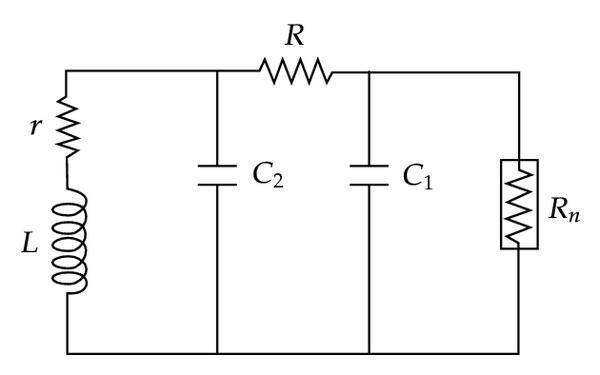
\includegraphics[width=0.30\textwidth]{chua}
\label{fig:Chua}
\end{figure}

Si queremos obtener las ecuaciones que describen el circuito, podemos medir, por ejemplo, la diferencia de potencial de las capacitancias y la corriente en el inductor. Las ecuaciones diferenciales que determinan la evolución de estos valores están dadas a continuación \cite{Website}.\\


$$
\frac{dV_1}{dt} = \frac{1}{RC_1}[(V_2-V_1) - Rg(V_1)] $$\\$$
\frac{dV_2}{dt} = \frac{1}{RC_2}[(V_1-V_2) + RI	   ]  $$	\\$$
\frac{dI}{dt} =    \frac{-V_2}{L}			$$	

Aquí $g(V1)$ es una función no lineal que define el comportamiento del diodo de Chua. Esta función está definida a trozos de la siguiente manera:\\

$$
g(V_1) =
\left\{
	\begin{array}{lll}
		 m_0 V_1 + (m_0 - m_1)E  & \mbox{if } V_1 \leq -E \\
		 m_1 V_1	 & \mbox{if }  |V_1| < E \\
		 m_0 V_1 + (m_1 - m_0)E  & \mbox{if } V_1 \geq E \\

		 
	\end{array}
\right.
$$

Con estas ecuaciones es sencillo simular computacionalmente la dinámica del circuito, por lo que se puede probar computacionalmente, guiado por la teoría de las ecuaciones, con diferentes valores de resistencia, capacitancia e inductancia antes de desarrollar el circuito en físico. \\

En general, lo que hace caótico a este circuito, son las capacitancias que actúan como reservorios de energía que de alguna manera guarda la historia del circuito y en conjunto con el elemento no lineal, hacen que las pequeñas variaciones en los estados iniciales se retroalimenten y vayan adquiriendo mayor influencia en el circuito. La explicación del formalismo teórico que permite analizar formalmente el caos del circuito lo dejaremos como parte del proyecto.

\section{\label{sec:level1}Montaje experimental}
El circuito que armaremos es realmente sencillo y su diagrama se encuentra en la figura \ref{fig:Chua}. Sin embargo, debido al comportamiento caótico del sistema, se necesita mucha cautela al diseñarlo y armarlo. Por otra parte, debido a que no hay quien manufacture los diodos de Chua, este dispositivo debe ser montado por nosotros. Su diseño no es nada complicado y se puede apreciar en la figura \ref{fig:diodo}\cite{Website}. \\

\begin{figure}[!hb]
\caption{Diodo de Chua}
\centering
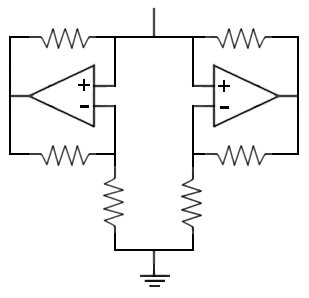
\includegraphics[width=0.30\textwidth]{diodo}
\label{fig:diodo}
\end{figure}

En general, solo se necesitarán diodos, resistencias, capacitores, e inductores para monta el circuito. El montaje puede ser hecho en una protoboard común y corriente, o puede ser un poco más sofisticado. Para hacer las mediciones del circuito solo será necesario un osciloscopio o dos (si se quiere observar la diferencia entre dos circuitos), y fuentes de potencial. Los valores de los elementos del circuito dependerán de lo que se quiera observar.

\section{\label{sec:level1}Cronograma}
El cronograma del proyecto está dado a grandes rasgos por: 

\begin{table}[!hb]
\centering
 \begin{tabular}{|p{6cm}|p{2cm}|} 
 \hline
 Descripción & Duración (Semanas) \\ [0.5ex] 
 \hline\hline
 Diseño del circuito y Simulaciones & 2\\
  \hline
 Montaje del circuito comprensión del caos en su modelo & 2\\
  \hline
 Toma de datos y verificación formal del caos & 3\\
  \hline
 Desarrollo del informe final & 2 \\
[1ex] 
 \hline
 \end{tabular}
 \caption{Cronograma del Desarrollo del Proyecto}
\end{table}

\section{\label{sec:level1}Resultados esperados}
 Debido a que el circuito es caótico, solo podemos decir a grandes rasgos lo que esperamos. Además de cumplir los objetivos generales, según las restricciones de la dinámica del circuito y lo que conocemos hasta ahora de la teoría \cite{Paper}, esperamos encontrar y medir los estados estables del sistema y compararlos con el valor teórico dado por los valores de resistencias, capacitancias e inductancias usadas; verificar la forma funcional en los distintos espacios definidos por la función a trozos que caracteriza el diodo de Chua; y medir la diferencia entre las trayectorias $(V_1, V_2, I)$ para cuantificar el caos del circuito y compararlo con los valores obtenidos por las simulaciones.\\
 
Entre más conozcamos sobre el análisis teórico de las ecuaciones características del circuito, podremos ampliar la lista de resultados cuantitativos esperados.\\

\begin{thebibliography}{99} 
\bibitem{Website}Valentin Siderskiy,{\it \ Chua's Circuit\ }{http://www.chuacircuits.com/}.\\ 
\bibitem{Paper} Michael Peter Kennedy,{\it Three steps to chaos- Part II: A Chua's circuit primer \ }{1993}\\ \end{thebibliography}


\end{document}
%
% ****** End of file apssamp.tex ******
